\RequirePackage{currfile}
\documentclass[12pt]{beamer}
\usepackage[utf8]{inputenc}
\usepackage[spanish]{babel}
\usepackage{standalone}
\usepackage{color}
\usepackage{siunitx}
\usepackage{hyperref}
%\hypersetup{colorlinks,linkcolor=,urlcolor=blue}
%\hypersetup{colorlinks,urlcolor=blue}
\usepackage{xcolor,soul}
\usepackage{etoolbox}
\usepackage{amsmath}
\usepackage{amsthm}
\usepackage{physics}
\usepackage{multicol}
\usepackage{bookmark}
\usepackage{longtable}
\usepackage{listings}
\usepackage{graphicx}
\usepackage{tikz}
\usetikzlibrary{patterns, matrix, backgrounds, decorations,shapes, arrows.meta}
\usepackage[autostyle,spanish=mexican]{csquotes}
\usepackage[os=win]{menukeys}
\usepackage{pifont}
\usepackage{pbox}
\usepackage{caption}
\captionsetup{font=scriptsize,labelfont=scriptsize}
%\usepackage[sfdefault]{roboto}  %% Option 'sfdefault' only if the base font of the document is to be sans serif

%Sección de definición de colores
\definecolor{ao}{rgb}{0.0, 0.5, 0.0}
\definecolor{bisque}{rgb}{1.0, 0.89, 0.77}
\definecolor{amber}{rgb}{1.0, 0.75, 0.0}
\definecolor{armygreen}{rgb}{0.29, 0.33, 0.13}
\definecolor{alizarin}{rgb}{0.82, 0.1, 0.26}
\definecolor{cadetblue}{rgb}{0.37, 0.62, 0.63}
\definecolor{deepblue}{rgb}{0,0,0.5}
\definecolor{brown}{rgb}{0.59, 0.29, 0.0}
\definecolor{OliveGreen}{rgb}{0,0.25,0}


\usefonttheme[onlymath]{serif}
%Sección de definición de nuevos comandos

\newcommand*{\TitleParbox}[1]{\parbox[c]{1.75cm}{\raggedright #1}}%
\newcommand{\python}{\texttt{python}}
\newcommand{\textoazul}[1]{\textcolor{blue}{#1}}
\newcommand{\azulfuerte}[1]{\textcolor{blue}{\textbf{#1}}}
\newcommand{\funcionazul}[1]{\textcolor{blue}{\textbf{\texttt{#1}}}}
\newcommand{\ptilde}[1]{\ensuremath{{#1}^{\prime}}}
\newcommand{\stilde}[1]{\ensuremath{{#1}^{\prime \prime}}}
\newcommand{\ttilde}[1]{\ensuremath{{#1}^{\prime \prime \prime}}}
\newcommand{\ntilde}[2]{\ensuremath{{#1}^{(#2)}}}
\renewcommand{\arraystretch}{1.5}

\newcounter{saveenumi}
\newcommand{\seti}{\setcounter{saveenumi}{\value{enumi}}}
\newcommand{\conti}{\setcounter{enumi}{\value{saveenumi}}}
\renewcommand{\rmdefault}{cmr}% cmr = Computer Modern Roman

\linespread{1.5}

\usefonttheme{professionalfonts}
%\usefonttheme{serif}
\DeclareGraphicsExtensions{.pdf,.png,.jpg}


%Sección para el tema de beamer, con el theme, usercolortheme y sección de footers
\mode<presentation>
{
  \usetheme{Warsaw}
  
  %\useoutertheme{infolines}
  \useoutertheme{default}
  \usecolortheme{spruce}
  \setbeamercovered{invisible}
  % or whatever (possibly just delete it)
  \setbeamertemplate{section in toc}[sections numbered]
  \setbeamertemplate{subsection in toc}[subsections numbered]
  \setbeamertemplate{subsection in toc}{\leavevmode\leftskip=3.2em\rlap{\hskip-2em\inserttocsectionnumber.\inserttocsubsectionnumber}\inserttocsubsection\par}
  \setbeamercolor{section in toc}{fg=blue}
  \setbeamercolor{subsection in toc}{fg=blue}
  \setbeamercolor{frametitle}{fg=blue}
  \setbeamertemplate{caption}[numbered]

  \setbeamertemplate{footline}
  \beamertemplatenavigationsymbolsempty
  \setbeamertemplate{headline}{}
}

\makeatletter
\setbeamercolor{section in foot}{bg=gray!30, fg=black!90!orange}
\setbeamercolor{subsection in foot}{bg=blue!30!yellow, fg=red}
\setbeamertemplate{footline}
{
  \leavevmode%
  \hbox{%
  \begin{beamercolorbox}[wd=.333333\paperwidth,ht=2.25ex,dp=1ex,center]{section in foot}%
    \usebeamerfont{section in foot} \insertsection
  \end{beamercolorbox}}%
  \begin{beamercolorbox}[wd=.333333\paperwidth,ht=2.25ex,dp=1ex,center]{subsection in foot}%
    \usebeamerfont{subsection in foot}  \insertsubsection
  \end{beamercolorbox}%
  \begin{beamercolorbox}[wd=.333333\paperwidth,ht=2.25ex,dp=1ex,right]{date in head/foot}%
    \usebeamerfont{date in head/foot} \insertshortdate{} \hspace*{2em}
    \insertframenumber{} / \inserttotalframenumber \hspace*{2ex} 
  \end{beamercolorbox}}%
  \vskip0pt%
\makeatother  

\makeatletter
\patchcmd{\beamer@sectionintoc}
  {\vfill}
  {\vskip\itemsep}
  {}
  {}
\makeatother


\title{\large{Tema 1 - Sistema de coordenadas curvilíneas}}
\subtitle{La física y la geometría}
\author{M. en C. Gustavo Contreras Mayén}
\date{\today}
\institute{Facultad de Ciencias - UNAM}
\titlegraphic{
\includegraphics[width=1.75cm]{../Imagenes/escudo-facultad-ciencias}\hspace*{4.75cm}~%
   
\includegraphics[width=1.75cm]{../Imagenes/escudo-unam}
}
\setbeamertemplate{navigation symbols}{}
\begin{document}
\maketitle
\fontsize{14}{14}\selectfont
\spanishdecimal{.}
\section*{Contenido}
\frame{\tableofcontents[currentsection, hideallsubsections]}
\section{Coordenadas curvilíneas}
\frame{\tableofcontents[currentsection, hideothersubsections]}
\subsection{Introducción}
\begin{frame}
\frametitle{Coordenadas curvilíneas}
La posición de un punto en el espacio tridimensional (con respecto a algún origen) generalmente se especifica al dar sus tres coordenadas cartesianas $(x, y, z)$ o, lo que es equivalente, al especificar el vector de posición $\vb{R}$ del punto.
\end{frame}
\begin{frame}
\frametitle{Coordenadas curvilíneas}
A menudo es más conveniente describir la posición del punto por otro conjunto de coordenadas más apropiadas para el problema en cuestión, los ejemplos comunes son coordenadas esféricas y cilíndricas.
\\
\bigskip
\pause
Estos son solo casos especiales de \emph{sistemas de coordenadas curvilíneas}, cuyas propiedades generales proponemos examinar en detalle.
\end{frame}
\begin{frame}
\frametitle{Funciones de la posición}
Supongamos que $q_{1}, q_{2}, q_{3}$ son funciones independientes de la posición, tales que
\begin{align}
\begin{aligned}
q_{1} &= q_{1} (x, y, z) \\
q_{2} &= q_{2} (x, y, z) \\
q_{3} &= q_{3} (x, y, z)
\end{aligned}
\label{eq:ecuacion_A_01_01}
\end{align}
\pause
o en términos de un vector de posición
\begin{align*}
q_{k} = q_{k}(\vb{R}) \hspace{1cm} k = 1, 2, 3
\end{align*}
\end{frame}
\begin{frame}
\frametitle{Jacobiano del sistema}
En las regiones donde el determinante Jacobiano
\begin{align}
\pdv{(q_{1}, q_{2}, q_{3})}{(x, y, z)} = 
\mdet{\displaystyle \pdv{q_{1}}{x} & \displaystyle \pdv{q_{1}}{y} & \displaystyle \pdv{q_{1}}{z} \\[1em]
\displaystyle \pdv{q_{2}}{x} & \displaystyle \pdv{q_{2}}{y} & \displaystyle \pdv{q_{2}}{z} \\[1em]
\displaystyle \pdv{q_{3}}{x} & \displaystyle \pdv{q_{3}}{y} & \displaystyle \pdv{q_{3}}{z} \\
}
\label{eq:ecuacion_A_01_02}
\end{align}
es diferente de cero, este sistema de ecuaciones se puede resolver simultáneamente para $x, y, z$
\end{frame}
\begin{frame}
\frametitle{Solución del sistema}
Obteniendo
\begin{align}
\begin{aligned}
x &= x (q_{1}, q_{2}, q_ {3}) \\
y &= y (q_{1}, q_{2}, q_ {3}) \\
z &= z (q_{1}, q_{2}, q_ {3})
\end{aligned}
\label{eq:ecuacion_A_01_03}    
\end{align}
o en términos de un vector
\begin{align*}
\vb{R} = \vb{R} (q_{1}, q_{2}, q_{3})
\end{align*}
\end{frame}
\begin{frame}
\frametitle{Jacobiano nulo}
Que el Jacobiano se anule implica que $q_{1}, q_{2}$ y $q_{3}$ son funciones no independientes, sino que están conectadas por una relación funcional de la forma $f (q_{1}, q_{2}, q_{3}) = 0$.
\\
\bigskip
De acuerdo con la ec.(\ref{eq:ecuacion_A_01_03}), asignarle valores numéricos para $q_{1}, q_{2}$ y $q_{3}$ conduce a un conjunto correspondiente de valores numéricos para $x, y, z$; es decir, localiza un punto $(x, y, z)$ en el espacio.
\end{frame}
\begin{frame}
\frametitle{Coordenadas curvilíneas}
De este modo, llegamos a considerar el conjunto de tres números $(q_{1}, q_{2}, q_{3})$ como las \emph{coordenadas curvilíneas} de un punto en el espacio.
\\
\bigskip
Es natural al tratar problemas físicos restringir la atención a los sistemas de coordenadas curvilíneas en los que cada punto en el espacio puede representarse al menos una vez dejando que $q_{1}, q_{2}$ y $q_{3}$ varíen sobre todos los valores posibles.
\end{frame}
\begin{frame}
\frametitle{Interpretación geométrica}
Las coordenadas curvilíneas tienen una interpretación geométrica simple.
\\
\bigskip
\pause
Si por el momento asignamos algún valor constante a $q_{k}$ tenemos
\begin{align*}
q_{k} (x, y, z) = \mbox{ constante} \hspace{0.5cm} (k = 1, 2, 3)
\end{align*}
que describe una superficie en el espacio.
\end{frame}
\begin{frame}
\frametitle{Interpretación geométrica}
Al asignar una serie de valores diferentes a $q_{k}$, generamos una \emph{familia de superficies} en las que $q_{k}$ es constante.
 \\
 \bigskip
Si las funciones se han elegido correctamente, hay al menos una superficie que pertenece a cada una de las tres familias que pasa por cualquier punto arbitrario $P$ en el espacio.
\end{frame}
\begin{frame}
\frametitle{Interpretación geométrica}
Por lo tanto, un punto en el espacio se caracteriza por la intersección de las tres superficies, $q_{1} = \mbox{ constante}, q_{2} = \mbox{ constante}, q_{3} = \mbox{ constante}$ (ver la figura \ref{fig:figura_A_01}), denominadas \emph{superficies coordenadas}.
\end{frame}
\begin{frame}[label=figura_01]
\frametitle{Sistema de coordenadas curvilíneas}
\begin{figure}[H]
   \centering
   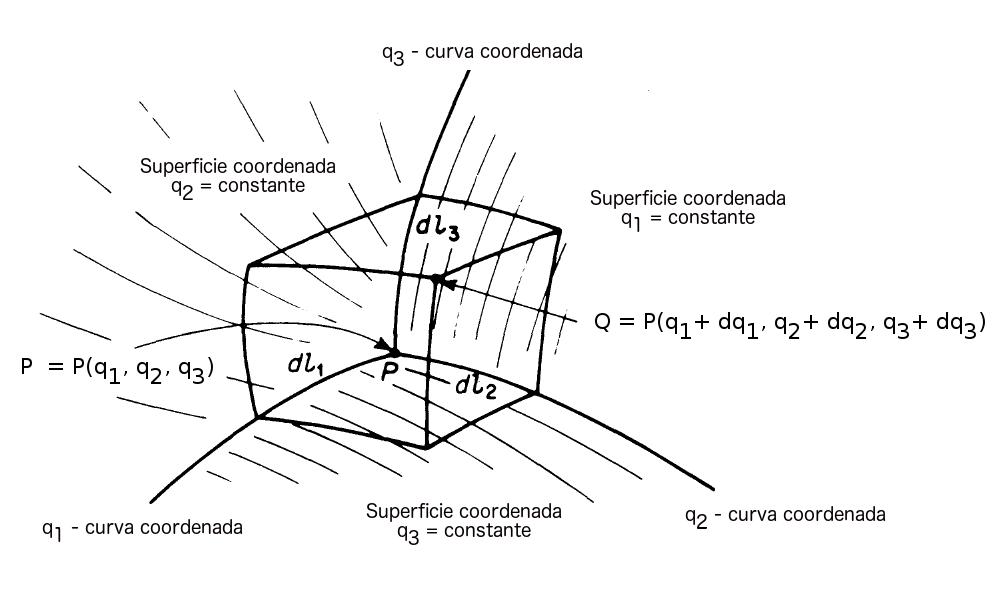
\includegraphics[scale=0.28]{Imagenes/CoordenadasCurvilineas_01.png}
   \caption{Sistema de coordenadas curvilíneas.}
   \label{fig:figura_A_01}
\end{figure}
\end{frame}
\begin{frame}
\frametitle{Interpretación geométrica}
Se llama \emph{superficie coordenada} para esa coordenada que es \underline{constante}, las otras dos coordenadas son variables a lo largo de esa superficie.
\end{frame}
\begin{frame}
\frametitle{Curva coordenada}
La intersección de dos superficies coordenadas da como resultado una curva sesgada denominada \emph{curva coordenada}.
\\
\bigskip
Por ejemplo, la intersección de las superficies coordenadas $q_{2}$ y $q_{3}$ da como resultado la curva de coordenadas etiquetada $q_{1}$.
\end{frame}
\begin{frame}
\frametitle{Curva coordenada}
Como esta curva se encuentra simultáneamente en las superficies $q_{2}$ = constante y $q_{3}$ = constante, solo $q_{1}$ varía a medida que avanzamos a lo largo de la curva; de ahí, que se le llame curva coordenada $q_{1}$.
\end{frame}
\begin{frame}
\frametitle{Coordenadas cartesianas}
En el caso especial de coordenadas cartesianas, las superficies coordenadas constan de tres planos mutuamente perpendiculares; las curvas coordenadas consisten en tres líneas perpendiculares entre sí.
\end{frame}
\begin{frame}
\frametitle{Distancia sobre las curvas}
En coordenadas cartesianas, los diferenciales $\dd{x}, \dd{y}, \dd{z}$ corresponden a distancias medidas a lo largo de cada una de las tres curvas coordenadas cartesianas.
\\
\bigskip
Los diferenciales análogos en coordenadas curvilíneas, $\dd{q_{1}}, \dd{q_{2}}, \dd{q_{3}}$, no tienen necesariamente una interpretación similar.
\end{frame}
\begin{frame}
\frametitle{Distancia sobre las curvas}
Como en la figura \ref{fig:figura_A_01}, sea $\dd{l_{1}}$ la distancia medida a lo largo de la curva $q_{1}-$coordenada desde el punto $P (q_{1}, q_{2}, q_{3})$ al punto vecino $(q_{1} + \dd{q_{1}}, q_{2}, q_{3})$.
\end{frame}
\againframe<2>{figura_01}
\begin{frame}
\frametitle{Distancia sobre las curvas}
Se aplica la misma definición para $\dd{l_{2}}$ y $\dd{l_{3}}$. Definimos las tres cantidades:
\begin{align}
h_{k} =  \abs{\dv{q_{k}}{l_{k}}} > 0, \hspace{1cm} k = 1, 2, 3
\label{eq:ecuacion_A_01_04}    
\end{align}
Esas cantidades (o variantes de ellas) se llaman \emph{coeficientes métricos}.
\end{frame}
\begin{frame}
\frametitle{Coeficientes métricos}
Son propiedades intrínsecas de cualquier sistema particular de coordenadas curvilíneas y en general, son funciones de la posición:
\begin{align*}
h_{k} = h_{k} (q_{1}, q_{2}, q_{3})
\end{align*}
\end{frame}
\begin{frame}
\frametitle{Vectores unitarios}
Sean $\vu{i}_{1}, \vu{i}_{2}$ y $\vu{i}_{3}$ los vectores unitarios que son tangentes a las curvas coordenadas $q_{1}$, $q_{2}$, $q_{3}$ respectivamente, en las direcciones en las que $q_{k}$ algebraicamente se incrementan, ver la figura \ref{fig:figura_A_02}.
\end{frame}
\begin{frame}
\frametitle{Vectores unitarios}
\begin{figure}[H]
    \centering
    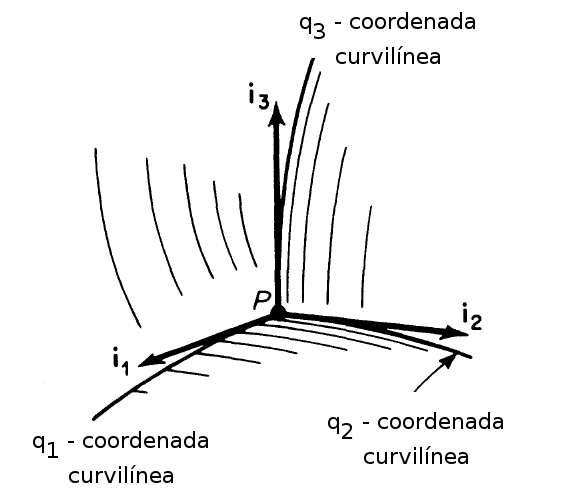
\includegraphics[scale=0.3]{Imagenes/CoordenadasCurvilineas_02.png}
    \caption{Vectores unitarios tangentes.}
    \label{fig:figura_A_02}
\end{figure}
\end{frame}
\begin{frame}
\frametitle{Vectores unitarios}
Es evidente que esos vectores unitarios tangentes están dados por
\begin{align}
\vu{i}_{k} = \pdv{\vb{R}}{l_{k}} \hspace{1cm} k = 1, 2, 3
\label{eq:ecuacion_A_01_05}    
\end{align}
\pause
Mientras que las \emph{magnitudes} de estos vectores unitarios son necesariamente constantes
\begin{align}
\vu{i}_{k} \cdot \vu{i}_{k} =  1 \hspace{1cm} \mbox{o} \hspace{1cm} \abs{\vu{i}_{k}} = 1
\label{eq:ecuacion_A_01_06}
\end{align}
\end{frame}
\begin{frame}
\frametitle{Vectores unitarios}
No se sigue que sus \emph{direcciones} permanezcan constantes de un punto a otro, por lo que los vectores unitarios son en general, funciones de la posición:
\begin{align*}
\vu{k} = \vu{i}_{k} (q_{1}, q_{2}, q_{3})
\end{align*}
\end{frame}
\begin{frame}
\frametitle{Vectores unitarios}
Se dice que los tres vectores unitarios no coplanares $\vu{1}, \vu{i}_{2}, \vu{i}_{3}$, constituyen un conjunto base de vectores unitarios para el sistema particular de coordenadas curvilíneas.
\end{frame}
\begin{frame}
\frametitle{Vectores unitarios}
Cualquier vector arbitrario, $\vb{u}$, puede expresarse de forma única en términos de ellos por una relación de la forma
\begin{align*}
\vb{u} = \vu{i}_{1} \, u_{1} + \vu{i}_{2} \, u_{2} + \vu{i}_{3} \, u_{3}
\end{align*}
\end{frame}
\begin{frame}
\frametitle{Vectores unitarios}
Un simple cálculo muestra que
\begin{align*}
u_{1} &= \dfrac{\vb{u} \cdot \vu{i}_{2} \cp \vu{i}_{3}}{\vu{i}_{1} \cdot \vu{i}_{2} \cp \vu{i}_{3}} \\[1em]
u_{2} &= \dfrac{\vu{i}_{1} \cdot \vb{u} \cp \vu{i}_{3}}{\vu{i}_{1} \cdot \vu{i}_{2} \cp \vu{i}_{3}} \\[1em]
u_{3} &= \dfrac{\vu{i}_{1} \cdot \vu{i}_{2} \cp \vb{u}}{\vu{i}_{1} \cdot \vu{i}_{2} \cp \vu{i}_{3}}
\end{align*}
\end{frame}
\begin{frame}
\frametitle{Vectores unitarios}
Al combinar las ecs. (\ref{eq:ecuacion_A_01_04}) y (\ref{eq:ecuacion_A_01_05}), se obtiene
\begin{align}
\vu{i}_{k} = h_{k} \, \pdv{\vb{R}}{q_{k}}
\label{eq:ecuacion_A_01_07}
\end{align}
\end{frame}
\begin{frame}
\frametitle{Vectores unitarios}
Esta expresión nos proporciona una fórmula alterna para calcular los coeficientes métricos
\begin{align}
h_{k} = \dfrac{1}{\abs{\pdv*{\vb{R}}{q_{k}}}}
\label{eq:ecuacion_A_01_08}    
\end{align}
\pause
La utilidad de esta expresión particular reside en el cálculo de los coeficientes métricos para sistemas de coordenadas curvilíneas definidos explícitamente por la ec. (\ref{eq:ecuacion_A_01_03}).
\end{frame}
\begin{frame}
\frametitle{Vectores unitarios}
Así, si ponemos:
\begin{align*}
\vb{R} = \vu{i} \, x + \vu{j} \, y + \vu{k} \, z
\end{align*}
por lo que es evidente que:
\begin{align*}
\pdv{\vb{R}}{q_{k}} = \vu{i} \, \pdv{x}{q_{k}} + \vu{j} \, \pdv{y}{q_{k}} + \vu{k} \, \pdv{z}{q_{k}}
\end{align*}
\end{frame}
\begin{frame}
\frametitle{Vectores unitarios}
Y de aquí:
\begin{align}
\begin{aligned}
\dfrac{1}{h_{k}^{2}} &= \left( \pdv{x}{q_{k}} \right)^{2} + \left( \pdv{y}{q_{k}} \right)^{2} + \left( \pdv{z}{q_{k}} \right)^{2}  \\
{}& \hspace{2cm} k = 1, 2, 3
\end{aligned}
\label{eq:ecuacion_A_01_09}
\end{align}
\pause
Por ejemplo, en coordenadas cartesianas donde $q_{1} = x, q_{2} = y, q_{3} = z$, se encuentra que $h_{1} = h_{2} = h_{3} = 1$.
\end{frame}

\end{document}